%------------------------------------------------
\section{Optimization results}
%------------------------------------------------
\begin{frame}[t]
	\frametitle{Optimization results}
	\tikzstyle{background grid}=[draw, black!50,step=.5cm]
	%
	\uncover<1->{StoMADS, \texttt{NOMAD}\ifshowcitations\footpartcite{NOMAD}\fi, and genetic algorithms were used to solve the problem\ifshowcitations\footpartcite{Alhandawi2021b}\fi}\\
	%
	\begin{columns}[t] % The "c" option specifies centered vertical alignment while the "t" option is used for top vertical alignment
		\begin{column}{.42\textwidth} % Left column and width
			\vspace{-1.2em}
			% Optimization problem
			\begin{exampleblock}{Objective and constraints}
				\vspace{-1.2em}
				\begin{equation*}
					\begin{aligned}
						& \underset{\mathbf{x}}{\text{min}}
						& & f(\mathbf{x}) = \mathbb{E}_{\Theta}\left[{f}_{\Theta}(\mathbf{x}) = -M^{T}\right]\\
						& \text{subject to}
						& & {c}(\mathbf{x}) = \mathbb{E}_{\Theta}\left[{c}_{\Theta}(\mathbf{x}) \equiv n_{I,\text{max}} - H_{\text{max}}\right] \le 0\\
						& \text{where}
						& & \mathbf{x}=\left[n_E,S_D,n_T\right]^\mathit{T},\Theta\mathrm{:realizations}
					\end{aligned}
				\end{equation*}
			\end{exampleblock}
			\vspace{-0.5em}
			% Variables
			\begin{alertblock}{Design variables}
				\vspace{-0.0em}
					\begin{itemize}\itemsep0em
						\item $n_E:$ Number of essential workers
						\item $S_D:$ Social distancing factor
						\item $n_T:$ Number of tests daily
					\end{itemize}
			\end{alertblock}
			\vspace{-0.5em}
			% Parameters
			\begin{blueblock}{Randomly seeded parameters}
				\vspace{-0.0em}
				\begin{itemize}\itemsep0em
					\item Initial conditions
					\item Interactions, demographics
				\end{itemize}
			\end{blueblock}
		\end{column}
		%
		\begin{column}{.5\textwidth} % Left column and width
			\tikzstyle{background grid}=[draw, black!50,step=.5cm]
			\begin{tikzpicture}[remember picture, overlay]%[show background grid]
				\node [inner sep=0pt, opacity=1.0,minimum size=10cm]  at (0.47\textwidth,-0.05\textheight) (mobility) 
				{	
					\centering
					\only<2>{
\includegraphics[height=12pt]{results_opt_traces/legend_0.pdf}}%
					\only<3>{
\includegraphics[height=12pt]{results_opt_traces/legend_1.pdf}}%
					\only<4->{
\includegraphics[height=12pt]{results_opt_traces/legend_2.pdf}}%
				};
				\node [inner sep=0pt,above right, opacity=1.0]  at (0.0\textwidth,-0.69\textheight) (mobility) 
				{
					\only<2>{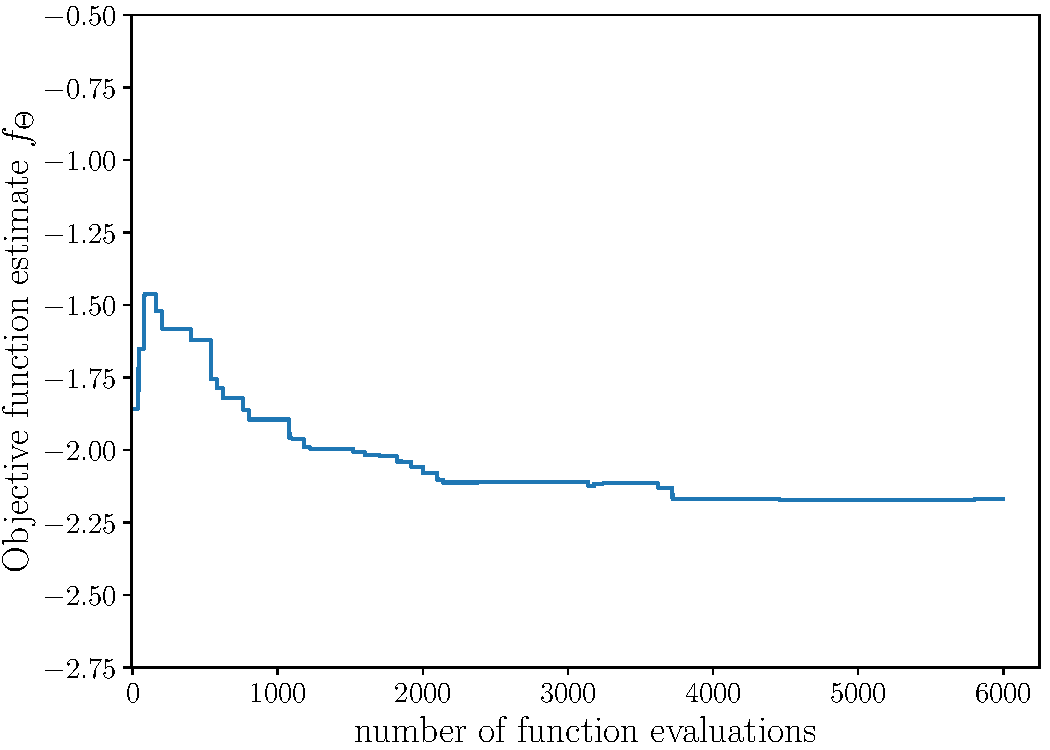
\includegraphics[width=0.95\textwidth]{results_opt_traces/f_nk=20_0.pdf}}%
					\only<3>{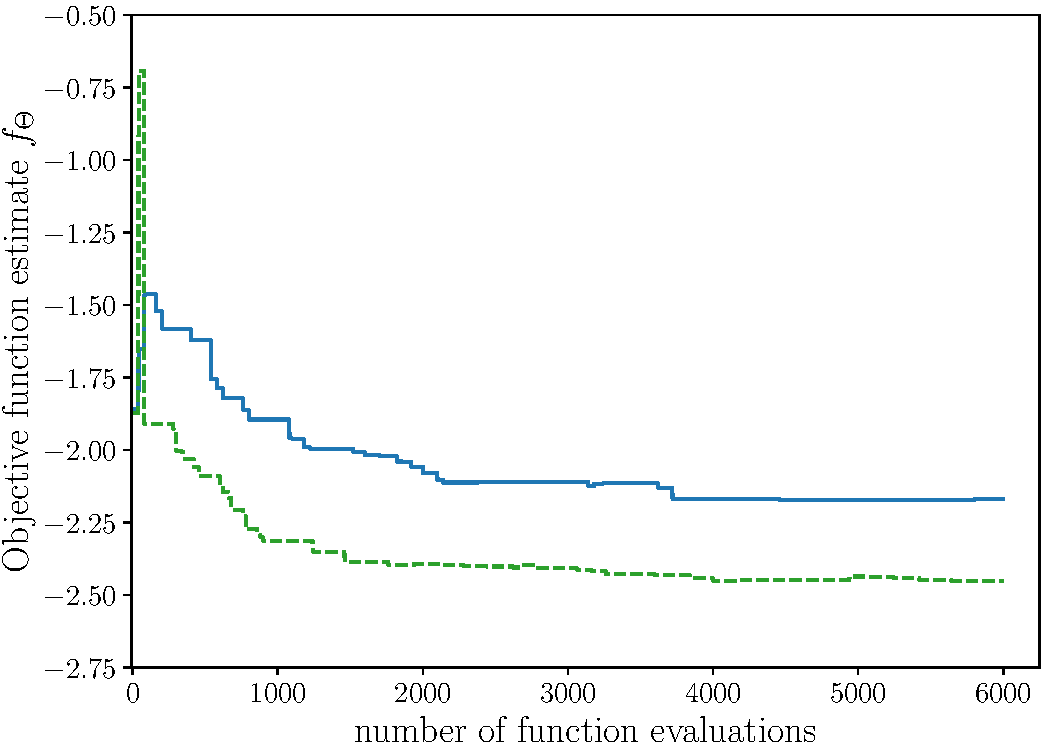
\includegraphics[width=0.95\textwidth]{results_opt_traces/f_nk=20_1.pdf}}%
					\only<4>{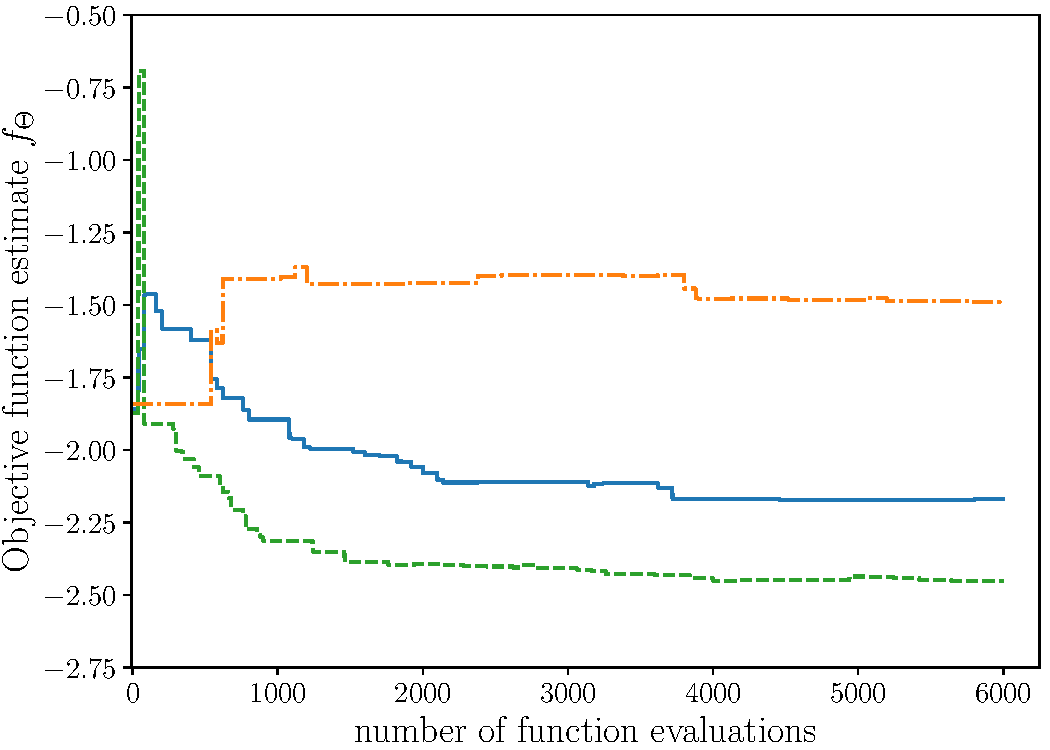
\includegraphics[width=0.95\textwidth]{results_opt_traces/f_nk=20_2.pdf}}%
					\only<5>{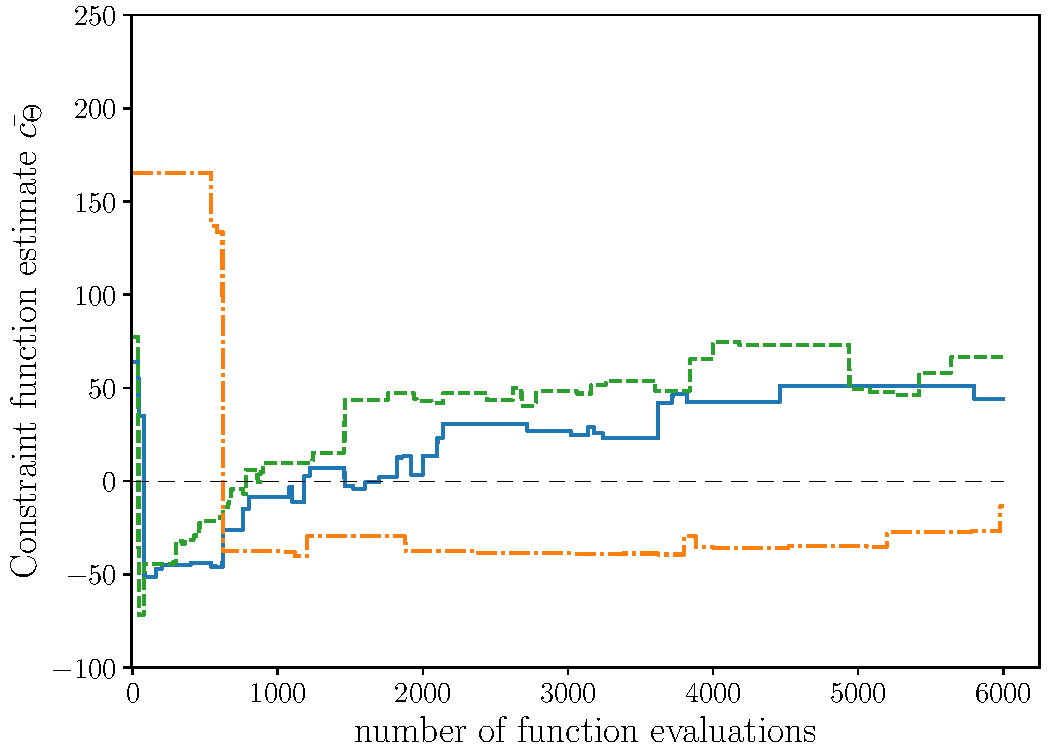
\includegraphics[width=0.95\textwidth]{results_opt_traces/g_nk=20_2.pdf}}%
				};
				\only<2-5>{
					\node[inner sep=0pt,align=flush center,above=\belowcaptionskip of mobility,text width=\linewidth]
					{\vspace{1em}{
						\large sampling rate $n^k=4$
					}};
				}%
				% show origin
				% \fill (0,0) circle (2pt);
			\end{tikzpicture}%
			\begin{tikzpicture}[remember picture, overlay]%[show background grid]
				\node [inner sep=0pt,above right, opacity=1.0]  at (0.0\textwidth,-0.75\textheight) (mobility) 
				{
					\only<6>{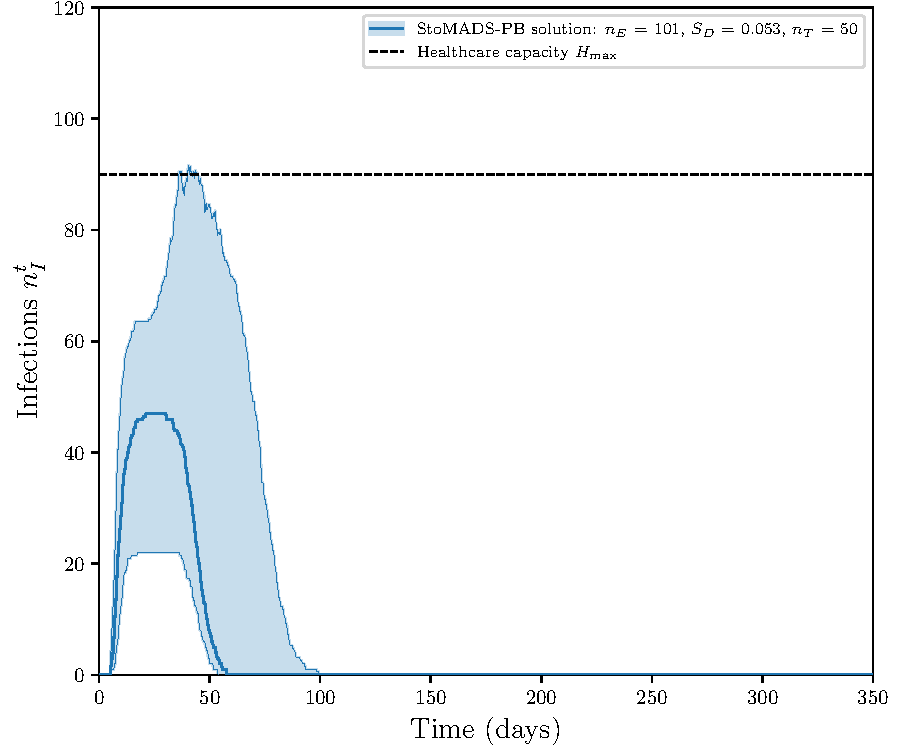
\includegraphics[width=0.93\textwidth]{trajecctory_results/I_compare_opt_0.pdf}}%
					\only<7>{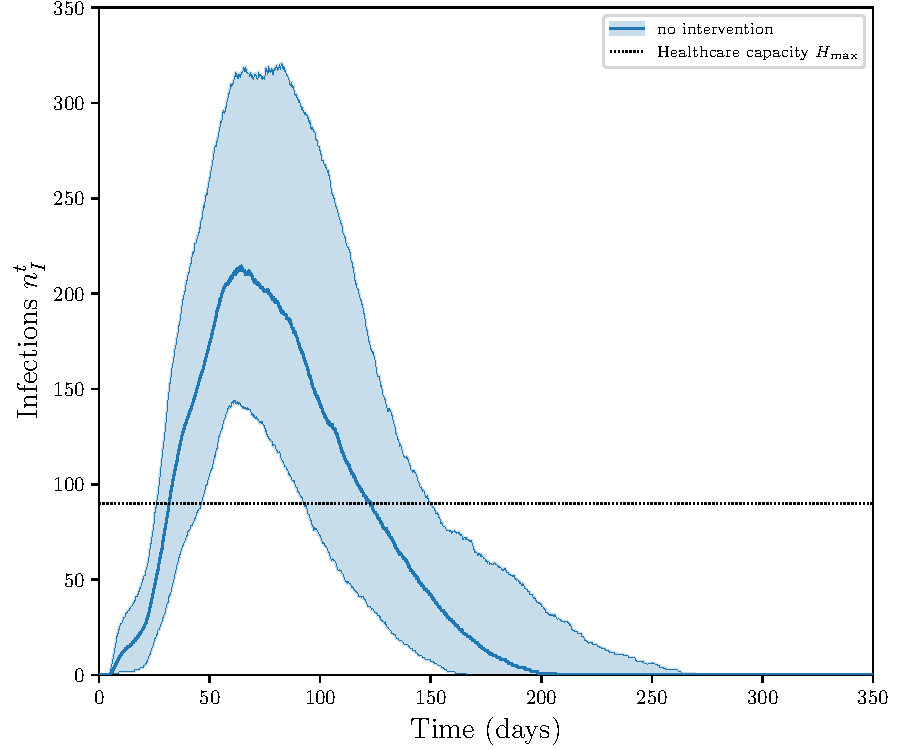
\includegraphics[width=0.93\textwidth]{trajecctory_results/I_compare_opt_1.pdf}}%
					\only<8>{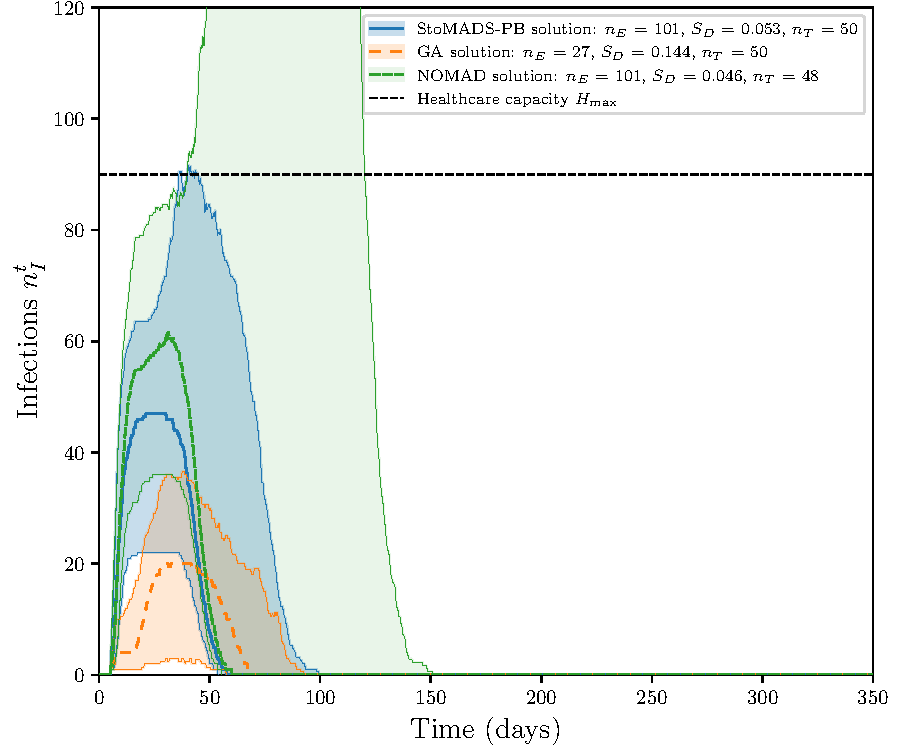
\includegraphics[width=0.93\textwidth]{trajecctory_results/I_compare_opt_2.pdf}}%
					\only<9>{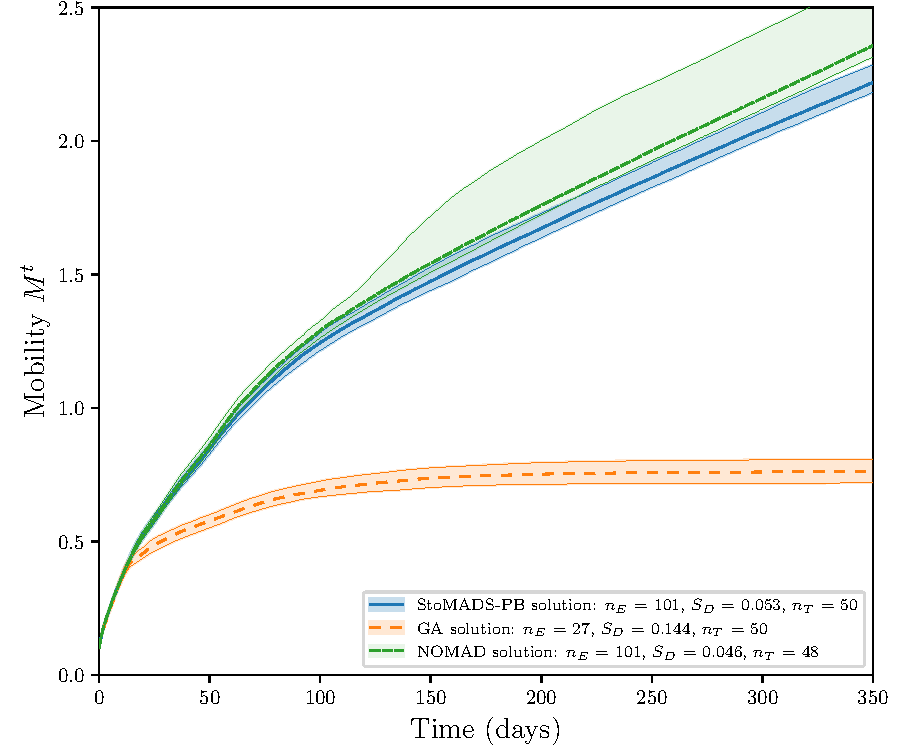
\includegraphics[width=0.93\textwidth]{trajecctory_results/M_compare_opt_2.pdf}}%
				};
				\only<6->{
					\node[inner sep=0pt,align=flush center,above=\belowcaptionskip of mobility,text width=\linewidth]
					{\vspace{1em}{
						\large best known solution
					}};
				}%
				% show origin
				% \fill (0,0) circle (2pt);
			\end{tikzpicture}%
		\end{column}
	
	\end{columns}
	\vspace{-3em}
\end{frame}
\addtocounter{footnote}{-2}
%------------------------------------------------